%==========================オプションおよび文書クラスの設定==========================
%"autodetect-engine"-どのエンジンでもコンパイル可能にするオプション
%"dvipdfmx-if-dvi"-必要な場合のみdvipdfmx経由のpdf化をするオプション(LuaTeXやXeTeXはPDFに直接変換するため)
%"ja=standard"-日本語文書の標準設定を利用するオプション
%"bxjs…"-どのエンジンでも利用可能なドキュメントクラス
%--以下のいずれかを選択--
\documentclass[autodetect-engine,dvipdfmx-if-dvi,ja=standard,a4paper,11pt]{bxjsarticle} %章の無いレポート
%\documentclass[autodetect-engine,dvipdfmx-if-dvi,ja=standard,a4paper,10pt]{bxjsslide} %スライド
%\documentclass[autodetect-engine,dvipdfmx-if-dvi,ja=standard,a4paper,10pt]{bxjsbook} %書籍
%\documentclass[autodetect-engine,dvipdfmx-if-dvi,ja=standard,a4paper,10pt]{bxjsreport} %章のある論文やレポート

%==============================プリアンブルの設定==============================
\title{研究会第一回} %タイトル
\author{B4 福田真悟} %著者名
\date{2020.4.28}%日付 %日付下の余白をN[mm]減らす

%///////////////////////////////////////////////////////////////////////////////////////////////////////////
%////////////////////////////////////パッケージの読込み及び設定の書換え//////////////////////////////////////
%///////////////////////////////////////////////////////////////////////////////////////////////////////////
\usepackage{graphicx} %図の挿入に関するパッケージ
\usepackage{float} %[H]で図の位置を固定する機能をONにするパッケージ
\usepackage{subcaption} %サブキャプションに関するパッケージ
\captionsetup{labelsep=space} %サブキャプション後の":"を非表示にする
\usepackage{enumerate} %{enumerate}[]の,[]の中の通りの箇条書きにすることができるパッケージ
\usepackage{amsmath} %数式に関するパッケージ
\usepackage{mathtools} %数式に関するパッケージ
\usepackage{bm} %ベクトル表示のコマンドを追加するパッケージ
\usepackage{comment} %複数行のコメントアウトを可能にするパッケージ
\usepackage{ascmac} %枠に関するパッケージ
\usepackage{tabularx} %表に関するパッケージ
\setpagelayout{top=10truemm,bottom=15truemm,left=15truemm,right=15truemm}  %余白に関する設定の書換え(bxjs…クラスではgeometryパッケージは使用不可)
\graphicspath{{../figures/}} %図を挿入する際に.texファイルの上の階層にあるfiguresというフォルダを参照可能にする
\usepackage{url}

%余白に関する設定の書換え(bxjs…クラスではgeometryパッケージは使用不可)
\belowcaptionskip=-0pt %キャプション下の余白をN[pt]減らす
\graphicspath{{../figures/}} %図を挿入する際に.texファイルの上の階層にあるfiguresというフォルダを参照可能にする

%使用記号の追加
\newcommand{\divergence}{\mathrm{div}\,}  %ダイバー
\newcommand{\grad}{\mathrm{grad}\,}  %グラディエント
\newcommand{\rot}{\mathrm{rot}\,}  %ローテーション

%\pagestyle{myheadings} %myheading文字列 emptyページ番号なし plainフッダーに
%\markright{\footnotesize 2月28日(金)15:00~ 顔合わせ}%全ページ共通への挿入
%================================以下本文================================
\begin{document}
\maketitle %設定したタイトルの挿入
\section{進捗状況}%sectionの前に*をつけると数字の振り分けが消える不思議
論文購読「A model of chaotic evolution of an ultrathin liquid film flowing down an inclined plane」
\section{低レイノルズ数における液膜流}
まずモデルの概要図を下記に示す.
\begin{figure}[H]%[h]は記述したところ。[t]はそのページの上端。[t]はそのページの下端、[p]はページいっぱい
\begin{center}
\includegraphics[width=.6\textwidth]{aboutNEW.jpg} 
\end{center}
\caption{斜面に沿った液膜流の概要図}%図名
\label{fig:about}%fig図tb表
\end{figure}
図\ref{fig:about}に示す角度$\alpha$に傾いた平らな斜面の上に流れる非常に薄く,レイノルズ数の小さい速度が遅い液膜流について考える.ここでの薄いは,流れのスケール($x$方向の長さ)に対して十分に無視できる厚さであり,レイノルズ数は${\rm Re}\ll1$とする.このとき慣性力を無視し,粘性力,重力,分子間力,表面張力が支配的になる.この液膜流に関しての1次元発展方程式を下記に示す.
\begin{equation}
\frac{\partial\phi}{\partial\tau}+\phi\frac{\partial\phi}{\partial\tilde{x}}+\frac{\partial^2\phi}{\partial\tilde{x}^2}+\frac{\partial^4\phi}{\partial\tilde{x}^4}=0
\label{eq:ks}
\end{equation}
この方程式をKuramoto-Sivashinsky方程式と呼ぶ.この式(\ref{eq:ks})の導出を下記にまとめる.


\subsection{Navier-Stokes方程式の簡略化}
まずNavier-Stokes方程式を下記に示す.
\begin{equation}
\begin{split}
\rho \left(\frac{\partial u}{\partial t}+u\frac{\partial u}{\partial x}+v\frac{\partial u}{\partial y}+w\frac{\partial u}{\partial z}\right)&=-\frac{\partial P}{\partial x}+\mu \left(\frac{\partial ^2u}{\partial x^2}+\frac{\partial^2 u}{\partial y^2}+\frac{\partial^2 u}{\partial z^2}\right)+F_x\\
\rho \left(\frac{\partial v}{\partial t}+u\frac{\partial v}{\partial x}+v\frac{\partial v}{\partial y}+w\frac{\partial v}{\partial z}\right)&=-\frac{\partial P}{\partial y}+\mu \left(\frac{\partial ^2v}{\partial x^2}+\frac{\partial ^2v}{\partial y^2}+\frac{\partial ^2v}{\partial z^2}\right)+F_y\\
\rho \left(\frac{\partial w}{\partial t}+u\frac{\partial w}{\partial x}+v\frac{\partial w}{\partial y}+w\frac{\partial w}{\partial z}\right)&=-\frac{\partial P}{\partial z}+\mu \left(\frac{\partial ^2w}{\partial x^2}+\frac{\partial ^2w}{\partial y^2}+\frac{\partial ^2w}{\partial z^2}\right)+F_z\\
\end{split}
\end{equation}
このときの$(x,y,z,t)$はそれぞれの位置と時間を表し,$(u,v,w)$は$(x,y,z)$それぞれの方向の速度を表している.$\rho$は液体の密度,$\mu$は粘性係数,$P$は圧力,$(F_x,F_y,F_z)$はそれぞれの方向にかかる外力を表している.また,液膜の厚さを$h$,重力加速度を$g$とする.これに加え,非圧縮流体の連続の式は,
\begin{equation}
\frac{\partial u}{\partial x}+\frac{\partial v}{\partial y}+\frac{\partial w}{\partial z}=0
\label{eq:mass}
\end{equation}
となる.\\
\ 条件として,${\rm Re}\ll1$と低レイノルズ数となっているので慣性力は無視できる.よって,$\frac{\partial u}{\partial t}=0,\frac{\partial v}{\partial t}=0$となる.二次元流れとなるので$w=0,\frac{\partial }{\partial z}=0,\frac{\partial ^2}{\partial z^2}=0$となる.膜は液膜流の長さに比べて十分に薄いため,$u\gg v$となる.よって,$u$に比べて$v$の影響は小さいので$v\simeq 0$とする.非圧縮の連続の式から$\frac{\partial u}{\partial x}=0$となる.外力は重力のみより,$F_x=mg\sin\alpha,F_y=-mg\cos\alpha$となる.圧力$P$から$y$方向に依存する$P_y=P_0+\rho g(h-y)\cos\alpha$を取り除くと,$\frac{\partial P_y}{\partial x}=\rho g\frac{\partial h}{\partial x}\cos\alpha\simeq0,\frac{\partial P_y}{\partial y}=\rho g\cos\alpha$となる.以上の条件から,Navier-Stokes方程式は下記のように簡略化できる.
\begin{equation}
\begin{split}
\mu\frac{\partial u^2}{\partial y^2}&=\frac{\partial P}{\partial x}-\rho g\sin\alpha\\
\frac{\partial P}{\partial y}&=0\\
\end{split}
\label{eq:simple}
\end{equation}
このときの近似をストークス近似という.

\subsection{圧力について}
圧力は,静水圧,分子間力,表面張力の3つ存在する.まず静水圧は,上記の$P_y$で表された値で下記に示す. 
\begin{equation}
P_y=P_0+\rho g(h-y)\cos\alpha
\end{equation}
この値に関しては既に考慮されているので除いて考える.分子間力より静水圧のほうが支配的であるときは,$\frac{\partial P_y}{\partial x}=\rho g\frac{\partial h}{\partial x}\cos\alpha$として考慮する必要がある.\\
\ 次に分子間力について考える.レナード--ジョーンズポテンシャルから近似解をフィッティングパラメータ(回帰分析による推定)を行う.圧力なので引力を正とすると,
\begin{equation}
P_m=\frac{A}{h^3}-\frac{B}{h^n}
\label{eq:pm1}
\end{equation}
となる.ここでの$A,B$はフィッティングパラメータである.$n$は$n>3$の整数である.$h(x,t)$は,座標$x$,時刻$t$における液膜厚さである.\\
\ 最後に表面張力について考える. 表面張力による圧力は,定数項を除くと,表面張力$\gamma$と表面の曲率の積となるので,
\begin{equation}
P_c=-\gamma \left[\frac{\partial^2 h}{\partial x^2}\left(1+\left(\frac{\partial h}{\partial x}\right)^2\right)^{-\frac{3}{2}}\right]
\label{eq:pc1}
\end{equation}
ここで液膜$h$は十分薄く,1より小さいので$\frac{\partial h}{\partial x}\ll 1$より,式(\ref{eq:pc1})は,
\begin{equation}
P_c=-\gamma\frac{\partial^2 h}{\partial x^2}
\label{eq:pc2}
\end{equation}
\ 以上の3つの力をまとめると,式(\ref{eq:pm1})と式(\ref{eq:pc2})との和を考え,
\begin{equation}
P=\frac{A}{h^3}-\frac{B}{h^n}-\gamma\frac{\partial^2 h}{\partial x^2}
\label{eq:pall}
\end{equation}
となる.この値を圧力として考える.

\subsection{$x$方向速度$u$の関数と流量の導出}
式(\ref{eq:simple})から速度の導出する.まず境界条件について,固体壁に接触する液体の相対速度は0となる.また,気体層と接触する流体に関しては,気体の粘性が液体の粘性より小さいことから近似的に速度勾配が0となる.以上をまとめると境界条件は,
\begin{equation}
\begin{split}
y&=0\ \rightarrow\ u=0\\
y&=h(x,t)\ \rightarrow\ 
\frac{\partial u}{\partial y}=0\\
\end{split}
\label{eq:BC1}
\end{equation}
となる.この境界条件をもとに式(\ref{eq:simple})の両辺を積分を行うと,
\begin{equation}
\frac{\partial u}{\partial y}=\left(\frac{\partial P}{\partial x}-\rho g\sin\alpha\right)\left(\frac{y}{\mu}+C_1\right)
\label{eq:u1}
\end{equation}
\begin{equation}
u=\left(\frac{\partial P}{\partial x}-\rho g\sin\alpha\right)\left(\frac{y^2}{2\mu}+C_1y+C_2\right)
\label{eq:u2}
\end{equation}
境界条件から,
\begin{equation}
C_1=-\frac{h}{\mu},C_2=0
\label{eq:u3}
\end{equation}
となる.よって,式(\ref{eq:u2})は,
\begin{equation}
u=\frac{1}{2}\left(\rho g\sin\alpha-\frac{\partial P}{\partial x}\right)\left(\frac{2hy}{\mu}-\frac{y^2}{2\mu}\right)
\label{eq:u4}
\end{equation}
となる.$z$方向1cmあたりの$x$方向の流量は,$u$の$y$方向積分で表される.流量$q$を下記に示す.
\begin{equation}
q=\displaystyle\int_{0}^{h(x,t)}u\ dy=\left(\rho g\sin\alpha-\frac{\partial P}{\partial x}\right)\frac{h^3}{3\mu}
\label{eq:q}
\end{equation}
よって流量が得られた.

\subsection{液膜流の質量保存}
質量保存則について,ある時刻での$x$方向の微小範囲で流出と流入の差分は,次の時刻における高さの増加量へと保存されている.これを式に表したものを下記に示す.
\begin{equation}
\frac{\partial h}{\partial t}+\frac{\partial q}{\partial x}=0
\end{equation}
この式の$q$に式(\ref{eq:q})を代入したものを下記に示す.
\begin{equation}
\begin{split}
&\frac{\partial h}{\partial t}+\frac{\rho g\sin\alpha}{\mu}h^2\frac{\partial h}{\partial x}\\
&+\left[\left(\frac{3A}{h^4}-\frac{nB}{h^{n+1}}\right)\frac{\partial h}{\partial x}+\gamma\frac{\partial^3 h}{\partial x^3}\right]\frac{h^2}{\mu}\frac{\partial h}{\partial x}\\
&+\left[\gamma\frac{\partial^4 h}{\partial x^4}-\left(\frac{12A}{h^5}-\frac{n(n+1)B}{h^{n+2}}\right)\left(\frac{\partial h}{\partial x}\right)^2+\left(\frac{3A}{h^4}-\frac{nB}{h^{n+1}}\right)\frac{\partial^2 h}{\partial x^2}\right]\frac{h^3}{3\mu}=0
\label{eq:heq}
\end{split}
\end{equation}
分子間力より静水圧のほうが支配的であるときは,$\frac{\partial P_y}{\partial x}=\rho g\frac{\partial h}{\partial x}\cos\alpha$として考慮した式(\ref{eq:heq})の非線形方程式を考える必要がある.

\subsection{$h$の標準化と長波近似}
液膜の厚さ$h$について,$h_0$を中心に標準化したものを下記に示す.
\begin{equation}
h=h_0(1+F)
\end{equation}
このときの$F$は$h_0$からの変化率を表している.このときの$F$は非常に微小で,長波近似より,$x$方向の変位に対して緩やかな変位と仮定すると,$F$の微分値も微小となる.$F^2$のオーダーを取ったものを下記に示す.ただし,十分な傾き$\alpha$があるとき,分子間力や表面張力の項は重力の項に比べて微小であるため,分子間力や表面張力の$F^2$も無視して考える.
\begin{equation}
\begin{split}
&\frac{\partial F}{\partial t}+\frac{\rho g\sin\alpha}{\mu}h_0^2\frac{\partial F}{\partial x}+\frac{2\rho g\sin\alpha}{\mu}h_0^2F\frac{\partial F}{\partial x}\\
&+\gamma\frac{h_0^3}{3\mu}\frac{\partial^4 F}{\partial x^4}+\left(\frac{3A}{h_0^4}-\frac{nB}{h_0^{n+1}}\right)\frac{h_0^3}{3\mu}\frac{\partial^2 F}{\partial x^2}=0
\label{eq:Feq}
\end{split}
\end{equation}


\subsection{ガリレイ変換}
式(\ref{eq:Feq})は,$\frac{\partial F}{\partial t}$の非定常の項と$\frac{\rho g\sin\alpha}{\mu}h_0^2\frac{\partial F}{\partial x}$の重力による項が他の項に比べて大きく,2つの項が釣り合っている.そこで座標系を重力による平均速度で移動する座標系に変換する.この変換をガリレイ変換という.ガリレイ変換した座標系$(x',t')$を下記に示す.
\begin{equation}
\begin{split}
x'&=x-\frac{\rho gh_0^2\sin\alpha}{\mu}t\\
t'&=t\\
\end{split}
\label{eq:gare1}
\end{equation}
この座標系における微分を下記に示す.
\begin{equation}
\begin{split}
\frac{\partial F}{\partial x}&=\frac{\partial F}{\partial x'}\frac{\partial x'}{\partial x}+\frac{\partial F}{\partial t'}\frac{\partial t'}{\partial x}\\
&=\frac{\partial F}{\partial x'}\\
\frac{\partial^n F}{\partial x^n}&=\frac{\partial^n F}{\partial x'^n}\\
\frac{\partial F}{\partial t}&=\frac{\partial F}{\partial x'}\frac{\partial x'}{\partial t}+\frac{\partial F}{\partial t'}\frac{\partial t'}{\partial t}\\
&=-\frac{\rho gh_0^2\sin\alpha}{\mu}\frac{\partial F}{\partial x'}+\frac{\partial F}{\partial t'}\\
\end{split}
\label{eq:gare2}
\end{equation}
式(\ref{eq:Feq})に式(\ref{eq:gare2})を代入したものを下記に示す.
\begin{equation}
\begin{split}
&\frac{\partial F}{\partial t'}+\frac{2\rho g\sin\alpha}{\mu}h_0^2F\frac{\partial F}{\partial x'}\\
&+\gamma\frac{h_0^3}{3\mu}\frac{\partial^4 F}{\partial x'^4}+\left(\frac{3A}{h_0^4}-\frac{nB}{h_0^{n+1}}\right)\frac{h_0^3}{3\mu}\frac{\partial^2 F}{\partial x'^2}=0
\label{eq:Feq2}
\end{split}
\end{equation}

\subsection{無次元化された方程式}
$F,x',t'$をそれぞれ代表値$F_0,L_0,t_0$で無次元化したもの下記に示す.
\begin{equation}
\begin{split}
\phi&=\frac{F}{F_0}\\
\tilde{x}&=\frac{x'}{L_0}\\
\tau&=\frac{t}{t_0}\\
\label{eq:norm}
\end{split}
\end{equation}
これを式(\ref{eq:Feq2})に代入し,各定数を下記に示すように設定する.
\begin{equation}
\begin{split}
\frac{2\rho gh_0^2\sin\alpha}{\mu}\frac{t_0F_0}{L_0}&=1\\
\gamma\frac{h_0^3}{3\mu}\frac{t_0}{L_0^4}&=1\\
\left(\frac{3A}{h_0^4}-\frac{nB}{h_0^{n+1}}\right)\frac{h_0^3}{3\mu}\frac{t_0}{L_0^2}&=1\\
\label{eq:para}
\end{split}
\end{equation}
以上の条件を満たすとき式(\ref{eq:Feq2})は,
\begin{equation}
\frac{\partial\phi}{\partial\tau}+\phi\frac{\partial\phi}{\partial\tilde{x}}+\frac{\partial^2\phi}{\partial\tilde{x}^2}+\frac{\partial^4\phi}{\partial\tilde{x}^4}=0
\label{eq:phieq}
\end{equation}
となる.よって式(\ref{eq:ks})が導出された.このKS方程式の時空構造を下記に示す.

\begin{figure}[H]%[h]は記述したところ。[t]はそのページの上端。[t]はそのページの下端、[p]はページいっぱい
\begin{center}
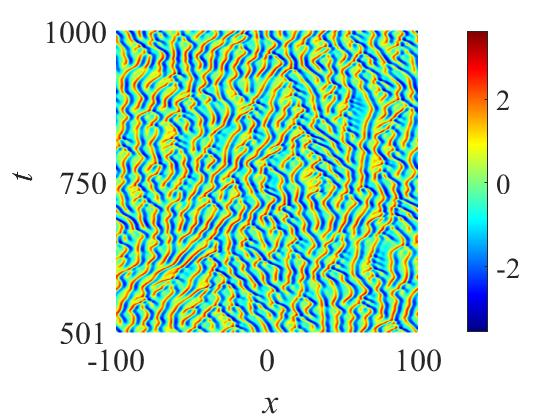
\includegraphics[width=.4\textwidth]{KS_result.jpg} 
\end{center}
\caption{KS方程式の結果}%図名
\label{fig:ks}%fig図tb表
\end{figure}



\section{今後の予定}
noisy?


%\begin{figure}[H]%[h]は記述したところ。[t]はそのページの上端。[t]はそのページの下端、[p]はページいっぱい
%\begin{center}
%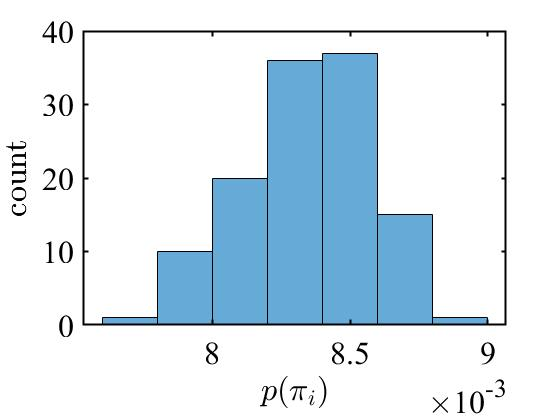
\includegraphics[width=.4\textwidth]{kadai3_histo.jpg}
%\end{center}
%\caption{課題3のヒストグラム(生成数は$100000$)}%図名
%\label{fig:kadai3_3}
%\end{figure}

%チェビシェフの不等式の置き換えの大数の弱法則から,
%\begin{equation}
%P(|\overline{X}_n-\mu|\ge \epsilon) \le \dfrac{\sigma^2}{n \epsilon^2}
%\end{equation}
%となる.ここでの$\overline{X}_n$はサンプルデータ$n$までの平均値(標本),$\mu$は理論的に考えられる平均値,$\epsilon$は許容誤差の大きさ,$\sigma$は標本データの分散である.




%$A^1$\cite{aaa}%参考文献



%\begin{itemize}
%\item アイテムコード1\\
%\item アイテムコード2\\
%\item アイテムコード3\\
%\item アイテムコード4\\
%\item アイテムコード5\\
%\end{itemize}


%\begin{figure}[H]%[h]は記述したところ。[t]はそのページの上端。[t]はそのページの下端、[p]はページいっぱい
%\begin{center}
%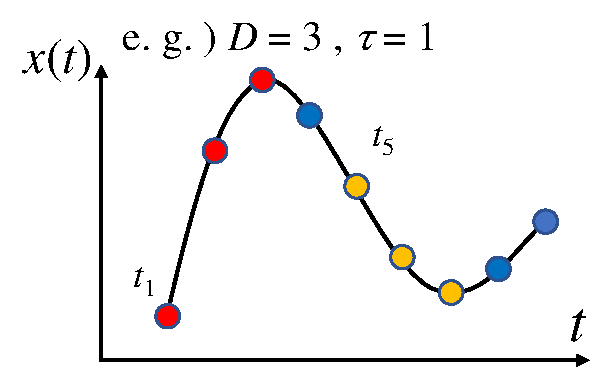
\includegraphics[width=.4\textwidth]{crop_PE1ver2.pdf} 
%\end{center}
%\caption{時系列$ x(t) $}%図名
%\label{fig:PE1}%fig図tb表
%\end{figure}

%\begin{eqnarray}
%\left\{%%{を作る
%\begin{array}{l}%l,llでは、lのときすべて{}の中の式のとき、{}の中にないものがあるならこっち
%\end{array}
%\right.
%\end{eqnarray} 


\begin{thebibliography}{9999}%参考文献
\bibitem{all}%参考文献citeするぞ
Boris Faybishenko, Alexander J. Babchin, Alexander L. Frenkel, David Halpern, Gregory I. Sivashinsky,"A
model of chaotic evolution of an ultrath", Colloids and Surfaces A,Physicochemical and Engineering Aspects,
192 (2001) 377$\sim$385
%\bibitem{re}
%カオス・フラクタル\ 講義ノート\ \#8,\url{https://ocw.hokudai.ac.jp/wp-content/uploads/2016/01/ChaosFractal-2011-Note-08.pdf}
%\bibitem{wgn}%参考文献citeするぞ
%ホワイトガウスノイズサンプルの生成-MATLAD wgn,\url{https://jp.mathworks.com/help/comm/ref/wgn.html}
%\bibitem{mutual}
%相互情報量の意味とエントロピーとの関係 | 高校数学の美しい物語,\url{https://mathtrain.jp/mutualinfo}
%\bibitem{net}
%複雑ネットワーク:統計物理学の視点,\url{http://mercury.yukawa.kyoto-u.ac.jp/~bussei.kenkyu/pdf/03/1/9999-031210.pdf}
\end{thebibliography}

%\newpage



\end{document}